\section{Design}
\subsection{CPU}
\begin{center}
\begin{figure}[H]
    \centering
\includegraphics[scale=0.40]{../grafik/overall_design.png}
\caption{Översiktlig design}
\label{fig:gui}
\end{figure}
\end{center}


\subsection{Grafik}
Grafikminnet kommer ett eget minnet med 256 ord à 16 bitar. För att utnyttja grafikminnet maximalt kommer den faktiska upplösningen vara 72x54. Detta leder till att vi behöver 3888 bitar för en bild och vi har 4096 tillgängliga i minnet. För att addressera grafikminnet så har vi en speciell instruktions STOREV som fungerar precis som STORE fast den skriver till grafikminnet. 
\begin{center}
\begin{figure}[H]
    \centering
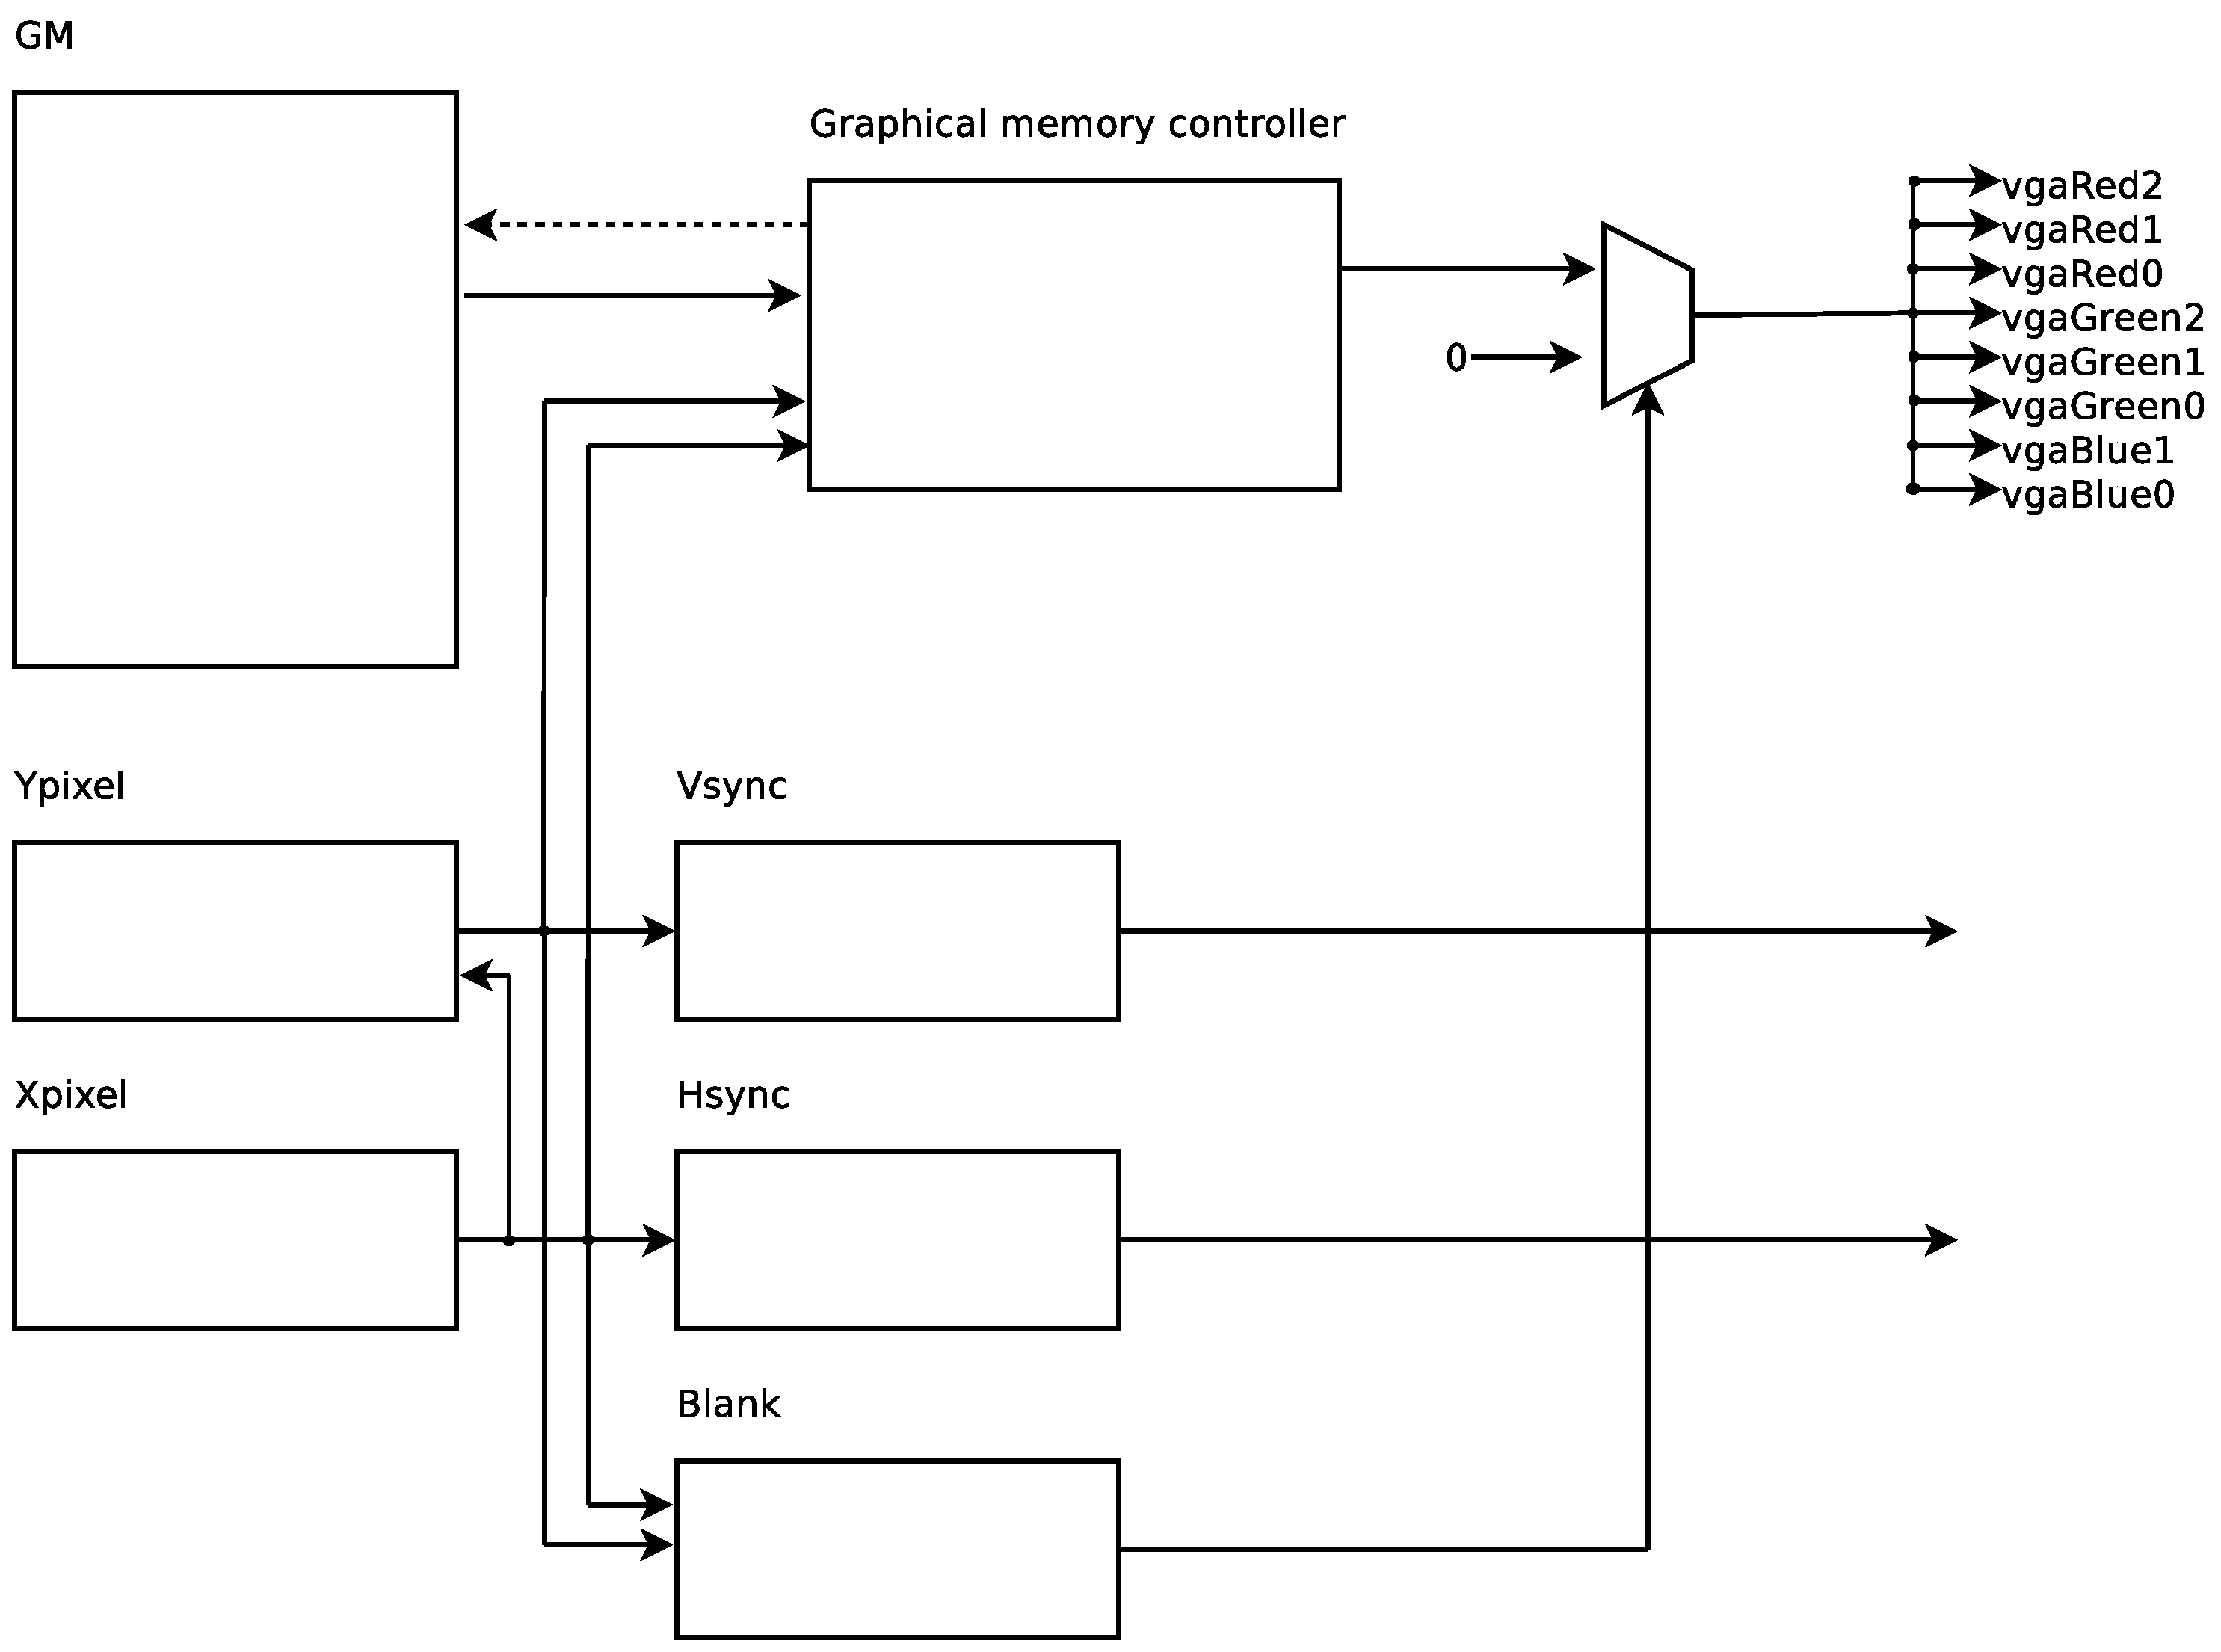
\includegraphics[scale=0.30]{../grafik/graphics.eps}
\caption{Översiktlig design}
\label{fig:gui}
\end{figure}
\end{center} 
\subsection{I/O enheter}
Processorn kommer ha en 8 bitars ingång och en 8 bitars utgång. Instruktionen IN GRx gör att man läser in de 8 bitarna till de 8 minst signifikanta bitarna på register GRx. OUT GRx skriver till utgången. Dessa två portar gör det möjligt att ha en extern 8 bitars ADC och en analog mux för att läsa av flera potentiometers som kommer användas som styrning av staplarna i PONG samt styra hastigheten av bollen. Detta möjliggör även för enklare ljud samt en resetknapp. 
\begin{center}
\begin{figure}[H]
    \centering
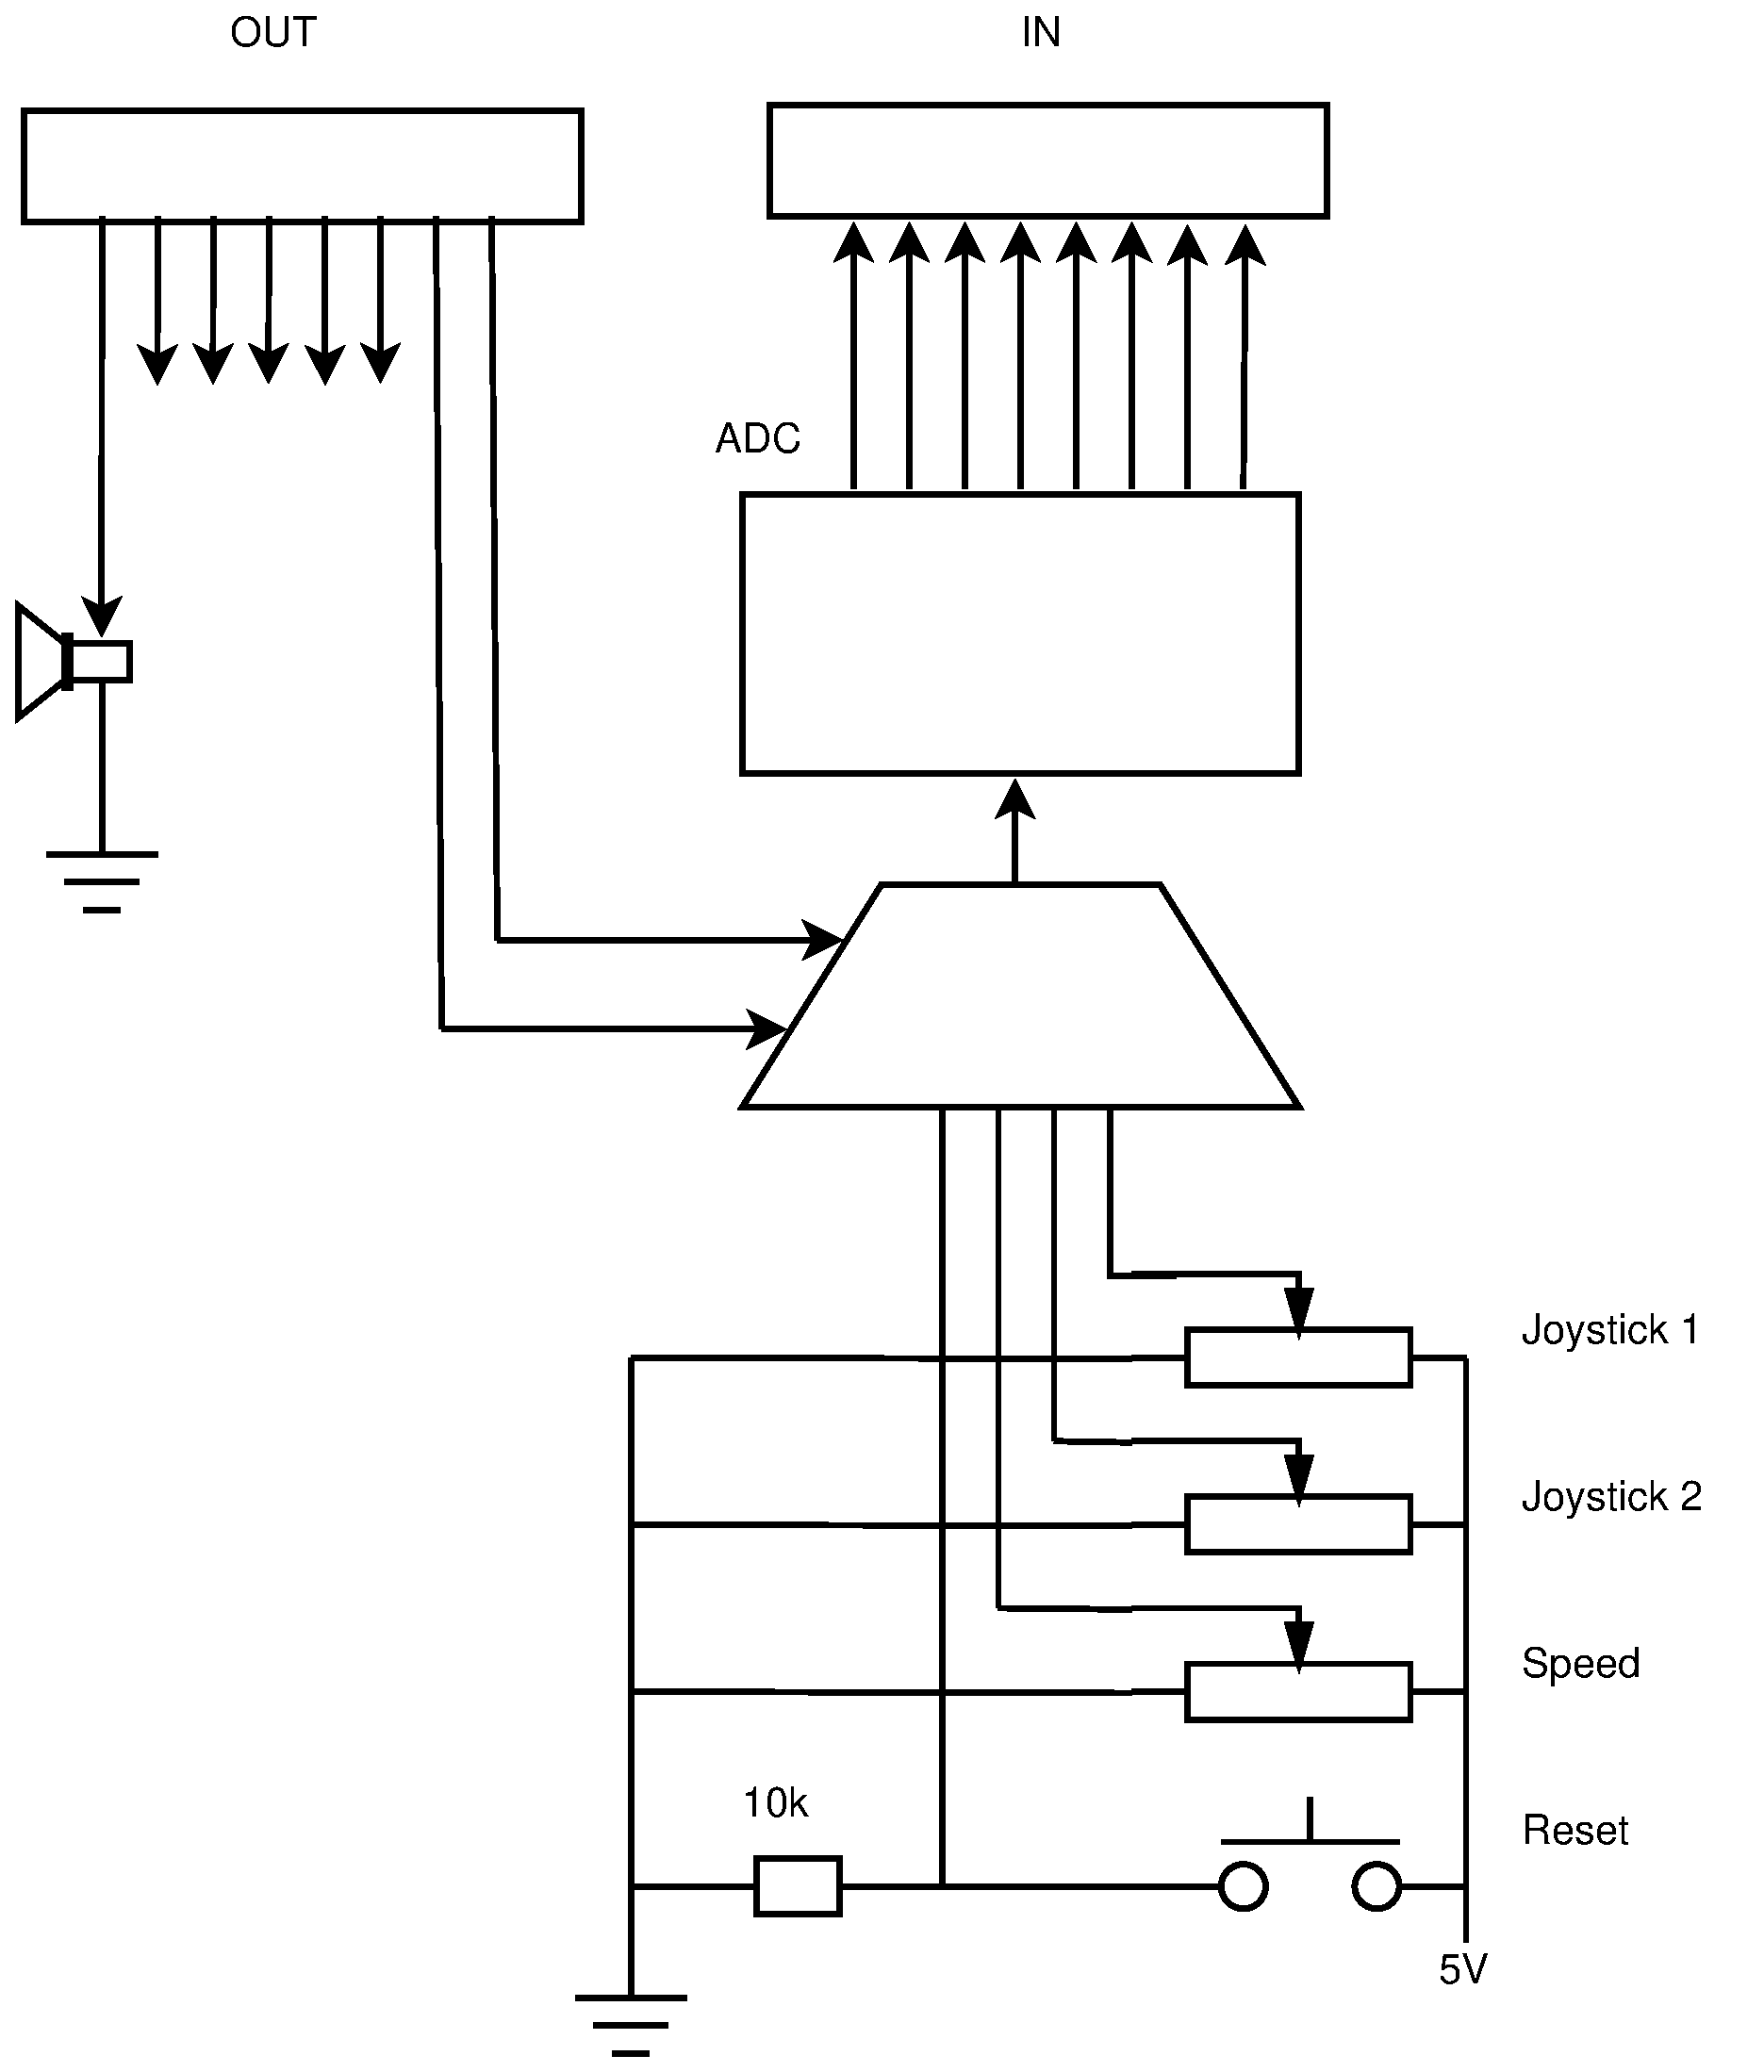
\includegraphics[scale=0.40]{../grafik/io.eps}
\caption{IO design}
\label{fig:gui}
\end{figure}
\end{center}
\subsection{Minnen}
Datorn kommer ha två minnet, dels ett delat programinne och dataminne och sedan ett grafikminne. Primärminnet kommer vara 16 bitar brett och ha 256 ord. Grafikminnet kommer vara likadant.
\subsection{Programmering}
Vi kommer göra en assembler(troligtvis i Python) som från en textfil direkt genererar VHDL kod som vi direkt kan kopiera in i koden för PM.